\section{Lesson 12 --- 17/11/2026}

\subsection{Hierarchical clustering}

With partitioning methods we organize the objects into $k$ exclusive groups, all at the same level. In many situations, however, we want to look at the data at \s{different levels} of granularity. Think of the employees of a company: we can split them into executives, managers and staff, and then split the staff again into senior officers, officers and trainees. Or think of handwritten digits: all the 7s form a group, but inside it we can find a subgroup of 7s written with the short horizontal line and a subgroup written without it. What we want here is not a single partition, but a \g{hierarchy} of clusters.

A \g{hierarchical clustering} method groups the data objects into a hierarchy, or ``tree'', of clusters. Sometimes the hierarchy is just a compact way to summarize and visualize the data; in other applications we really believe that the data have an underlying hierarchical structure that we want to discover (for example the evolutionary tree of species).

There are two directions to build the hierarchy:
\begin{itemize}
  \item \g{Agglomerative} (bottom-up): we start with $n$ singleton clusters, one per object, and we repeatedly \s{merge} the two nearest clusters, until all the objects are in a single cluster or a termination condition is met. Since each step merges two clusters into one, we need at most $n-1$ merges. The representative algorithm is \g{AGNES} (AGglomerative NESting).
  \item \g{Divisive} (top-down): we start with one cluster containing all the objects and we repeatedly \s{split} a selected cluster, until each cluster contains a single object or is coherent enough. The representative algorithm is \g{DIANA} (DIvisive ANAlysis).
\end{itemize}

\begin{center}
\begin{tikzpicture}[
  obj/.style={circle, draw, fill=blue!15, inner sep=1.5pt, minimum size=6mm},
  every node/.append style={font=\small}]
  % objects
  \foreach \n/\x in {a/0, b/1, c/2, d/3, e/4}
    \node[obj] (\n) at (\x,0) {$\n$};
  % agglomerative arrow
  \draw[-{Latex}, thick, blue!60!black] (-1,-0.3) -- (-1,3.3) node[midway, left, align=center] {AGNES\\merge};
  % divisive arrow
  \draw[-{Latex}, thick, red!60!black] (5,3.3) -- (5,-0.3) node[midway, right, align=center] {DIANA\\split};
  % levels
  \node[draw, rounded corners, minimum width=1.6cm, minimum height=6mm] at (0.5,1) {$ab$};
  \node[draw, rounded corners, minimum width=2.6cm, minimum height=6mm] at (3,1.8) {$cde$};
  \node[draw, rounded corners, minimum width=1.6cm, minimum height=6mm] at (3.5,1) {$de$};
  \node[draw, rounded corners, minimum width=4.6cm, minimum height=6mm] at (2,2.8) {$abcde$};
\end{tikzpicture}
\end{center}

In both cases the result is a \s{nested family of partitions}: every level of the tree is a partition of the data, and each cluster at one level is contained in a cluster of the level above. Notice that we don't need to fix $k$ to build the hierarchy: $k$ is needed only at the end, if we want to extract a flat partition from it.

\begin{remark}
The selection of the merge or split points is critical, because the decisions are \s{irreversible}: once two clusters are merged (or a cluster is split), the algorithm will never undo that step nor swap objects between clusters, as k-means or PAM do. If a decision is not well chosen, it propagates to all the following levels and may lead to low-quality clusters.
\end{remark}

\subsubsection{Distance between clusters: linkage}

To merge ``the two nearest clusters'' we need to define a distance between \s{sets} of objects, while what we have is a distance between single objects. We start from the pairwise dissimilarity matrix, computed with the point metric $d(x,y)$ that matches the data type (Euclidean, Manhattan, Jaccard, \dots), and we generalize it to clusters by aggregating all the cross-cluster distances:
\[
  d(C_1, C_2) = \operatorname{operation}\{\, d(x,y) : x \in C_1,\ y \in C_2 \,\}.
\]
This aggregation is called \g{linkage}. A linkage is not a new point distance: the point metric defines the local dissimilarity, the linkage defines what ``close clusters'' means. Changing either of the two choices may change the entire hierarchy.

\begin{definition}[Linkage measures]
Given two clusters $C_1$ and $C_2$, with $x \in C_1$ and $y \in C_2$:
\begin{itemize}
  \item \g{Single link} (minimum distance, nearest neighbor):
  \[
    d_s(C_1, C_2) = \min_{x \in C_1,\, y \in C_2} d(x,y);
  \]
  \item \g{Complete link} (maximum distance, farthest neighbor):
  \[
    d_c(C_1, C_2) = \max_{x \in C_1,\, y \in C_2} d(x,y);
  \]
  \item \g{Average link} (UPGMA, Unweighted Pair Group Method with Arithmetic Mean):
  \[
    d_a(C_1, C_2) = \frac{1}{|C_1|\,|C_2|} \sum_{x \in C_1} \sum_{y \in C_2} d(x,y).
  \]
\end{itemize}
\end{definition}

The three formulas differ only in the aggregation operator (min, max or mean), but this difference changes every later merge, because each one encodes a different notion of cluster shape.

\begin{center}
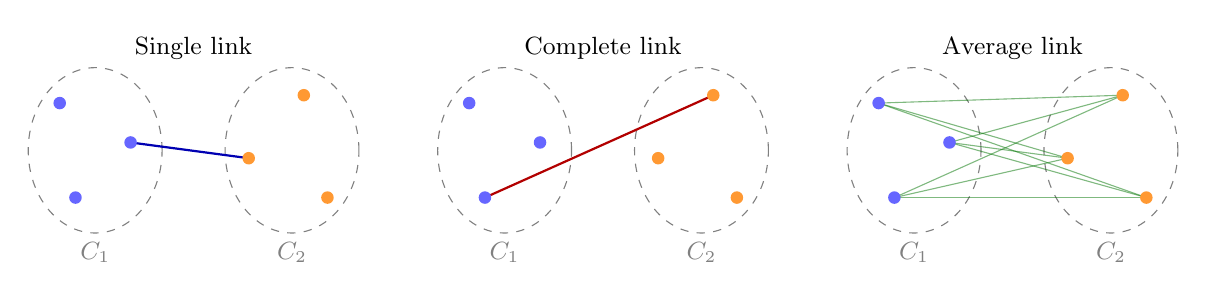
\begin{tikzpicture}[
  pt/.style={circle, fill=#1, inner sep=1.6pt},
  every node/.append style={font=\small}]
  \foreach \k/\title/\style in {0/Single link/blue!70!black, 1/Complete link/red!70!black, 2/Average link/green!45!black} {
    \begin{scope}[xshift=\k*5.2cm]
      \node at (2,2.3) {\title};
      \draw[gray, dashed] (0.75,1.0) ellipse (0.85 and 1.05);
      \draw[gray, dashed] (3.25,1.0) ellipse (0.85 and 1.05);
      \node[gray] at (0.75,-0.3) {$C_1$};
      \node[gray] at (3.25,-0.3) {$C_2$};
      \coordinate (p1) at (0.3,1.6);
      \coordinate (p2) at (0.5,0.4);
      \coordinate (p3) at (1.2,1.1);
      \coordinate (q1) at (2.7,0.9);
      \coordinate (q2) at (3.4,1.7);
      \coordinate (q3) at (3.7,0.4);
      \ifcase\k
        \draw[thick, \style] (p3) -- (q1);
      \or
        \draw[thick, \style] (p2) -- (q2);
      \or
        \foreach \p in {p1,p2,p3} \foreach \q in {q1,q2,q3}
          \draw[\style, opacity=0.5] (\p) -- (\q);
      \fi
      \foreach \p in {p1,p2,p3} \node[pt=blue!60] at (\p) {};
      \foreach \q in {q1,q2,q3} \node[pt=orange!80] at (\q) {};
    \end{scope}
  }
\end{tikzpicture}
\end{center}

\begin{itemize}
  \item \g{Single link} follows the \s{nearest bridge} between the two clusters. It can recover elongated or irregular (non-convex) structures, but it suffers from the \g{chaining effect}: a thin chain of points, for example noise, is enough to join two clusters that are clearly separated.
  \item \g{Complete link} controls the \s{farthest pair}. It tends to form compact clusters of similar size, but it breaks elongated groups and it is sensitive to extreme cross-cluster distances.
  \item \g{Average link} uses all the cross-cluster pairs, so it balances the local bridges of single link and the extreme pairs of complete link. It is often a useful compromise, but it can blur differences in density.
\end{itemize}

\begin{center}
\begin{tabular}{@{}llll@{}}
\toprule
Linkage & Main signal & Works well when\dots & Common pitfall \\
\midrule
Single & nearest bridge & clusters may be non-convex & chaining through noise \\
Complete & farthest pair & clusters are compact & breaks elongated groups \\
Average & all cross-pairs & a compromise is appropriate & can blur density differences \\
\bottomrule
\end{tabular}
\end{center}

There is no universally best linkage: the linkage is a \s{modeling assumption}, not a cosmetic parameter, and the right choice follows from the geometry we expect in the data and from the goal of the analysis. The same points can produce very different hierarchies with single, complete or average link, so it is good practice to inspect how sensitive the result is to the linkage, to the distance metric and to outliers. As usual, we must always scale the features before using a scale-sensitive distance.

\begin{remark}
The book lists a fourth measure, the \g{mean distance} $d_{mean}(C_1, C_2) = \norm{m_1 - m_2}$, i.e.\ the distance between the two centroids $m_1$ and $m_2$. It is the simplest to compute, but it needs a mean vector, so it cannot be used with categorical data, while the average link can. Watch out for the names: the slides call ``mean distance'' the average link $d_a$, while in the book ``mean distance'' is the centroid distance and $d_a$ is the ``average distance''.

The book also connects agglomerative clustering with k-means through \g{Ward's criterion}: merge the pair of clusters that gives the smallest increase of the SSE $E$ that k-means minimizes,
\[
  W(C_i, C_j) = \frac{n_i n_j}{n_i + n_j} \norm{m_i - m_j}^2,
\]
where $n_i = |C_i|$. All these linkages are special cases of a single update rule, the Lance--Williams formula.
\end{remark}

\subsubsection{Dendrogram}

The whole merge (or split) history is recorded in a tree called \g{dendrogram}:
\begin{itemize}
  \item the \s{leaves} are the individual observations;
  \item a \s{horizontal branch} represents a merge of two clusters;
  \item the \s{vertical position} of the branch, the \g{merge height}, is the linkage distance at which the merge happened.
\end{itemize}
A dendrogram must be read \s{vertically}: the merge height carries the dissimilarity information. The order of the leaves is chosen only for readability, so the horizontal gaps between leaves are not distances.

To turn the hierarchy into a flat partition we make a \g{horizontal cut}: the number of branches crossed by the cut is the number of clusters $k$. We can choose $k$ directly or choose a distance threshold; a large vertical gap between two consecutive merges suggests a stable cut, because the clusters stay the same for a wide range of thresholds.

\begin{center}
\begin{tikzpicture}[x=1.2cm, y=1.6cm, every node/.append style={font=\small}]
  % axis
  \draw[-{Latex}] (-0.5,0) -- (-0.5,3.5) node[above] {height};
  \foreach \h in {1,2,3} \draw (-0.55,\h) -- (-0.45,\h) node[left=2pt] {$\h$};
  % leaves
  \foreach \l/\x in {A/0, B/1, C/2, D/3, E/4} \node[below] at (\x,0) {$\l$};
  % merges
  \draw[thick] (0,0) -- (0,1) -- (1,1) -- (1,0);
  \draw[thick] (2,0) -- (2,1) -- (3,1) -- (3,0);
  \draw[thick] (0.5,1) -- (0.5,2) -- (2.5,2) -- (2.5,1);
  \draw[thick] (1.5,2) -- (1.5,3) -- (4,3) -- (4,0);
  % cut
  \draw[red!70!black, dashed, thick] (-0.3,1.5) -- (4.6,1.5) node[right] {cut $\Rightarrow k = 3$};
\end{tikzpicture}
\end{center}

\begin{remark}
A popular rule says that, to obtain $k$ clusters, we remove the $k-1$ longest links. This is the minimum-spanning-tree interpretation of \s{single link} (see below), not a universal dendrogram rule: with other linkages we simply cut the tree.
\end{remark}

\subsubsection{AGNES}

\g{AGNES} builds the full hierarchy bottom-up by repeatedly merging the nearest clusters:
\begin{enumerate}
  \item \s{Initialize}: create $n$ singleton clusters, one per object.
  \item \s{Search}: find the pair of clusters with minimum linkage distance.
  \item \s{Merge}: replace the pair by their union.
  \item \s{Update}: recompute the distances between the new cluster and all the remaining clusters.
  \item \s{Stop}: continue until there is one cluster, or $k$ clusters, or until the minimum distance exceeds a threshold.
\end{enumerate}
AGNES builds the entire hierarchy; $k$ is needed only when we want to extract a flat partition.

\paragraph{Single link and the minimum spanning tree.} Single link has a nice graph interpretation. Treat the observations as the vertices of a complete graph, where the edge between $x$ and $y$ has weight $d(x,y)$. Each single-link merge adds the \s{shortest edge connecting two different components}, which is exactly what Kruskal's algorithm does to build a \g{minimum spanning tree} (MST). So the ordered edges of the MST encode the whole single-link hierarchy, and cutting the $k-1$ longest MST edges gives $k$ clusters. This explains both why single link can be computed efficiently and why it chains: a short bridge between two groups is an MST edge like any other.

\paragraph{Complete link and the diameter.} The \g{diameter} of a cluster is the largest distance between two of its objects,
\[
  \operatorname{diam}(C) = \max_{x, y \in C} d(x,y).
\]
The complete-link distance between $C_1$ and $C_2$ is the largest cross-pair distance, so it is exactly the part of the diameter of $C_1 \cup C_2$ that the merge adds. For this reason complete link tends to minimize the increase of the cluster diameter at each merge. Single link, instead, accepts a short bridge even when the union becomes very wide.

\begin{example}[AGNES with single link]
We have five objects and the following dissimilarity matrix:
\begin{center}
\begin{tabular}{@{}c|ccccc@{}}
 & $A$ & $B$ & $C$ & $D$ & $E$ \\
\midrule
$A$ & 0 & 1 & 2 & 2 & 3 \\
$B$ & 1 & 0 & 2 & 4 & 3 \\
$C$ & 2 & 2 & 0 & 1 & 5 \\
$D$ & 2 & 4 & 1 & 0 & 3 \\
$E$ & 3 & 3 & 5 & 3 & 0 \\
\end{tabular}
\end{center}
\begin{enumerate}
  \item The smallest non-zero distance is $1$, and there is a tie: $A$ and $B$ are nearest neighbors, and so are $C$ and $D$. With the rule ``ties are merged at the same height'', both pairs merge at height $1$ and we obtain $\{AB\}, \{CD\}, \{E\}$.
  \item After every merge the distances must be recomputed. With single link we take the minimum over the cross pairs:
  \[
    \begin{aligned}
      d(AB, CD) &= \min\{2, 2, 2, 4\} = 2, \\
      d(AB, E) &= \min\{3, 3\} = 3, \\
      d(CD, E) &= \min\{5, 3\} = 3.
    \end{aligned}
  \]
  \begin{center}
  \begin{tabular}{@{}c|ccc@{}}
   & $AB$ & $CD$ & $E$ \\
  \midrule
  $AB$ & 0 & 2 & 3 \\
  $CD$ & 2 & 0 & 3 \\
  $E$ & 3 & 3 & 0 \\
  \end{tabular}
  \end{center}
  \item The next merge is $AB \cup CD = ABCD$ at height $2$.
  \item The final merge is $ABCD \cup E$ at height $3$, since $d(ABCD, E) = \min\{3, 3\} = 3$.
\end{enumerate}
The resulting dendrogram is the one shown in the previous section: the cut between heights $1$ and $2$ gives the three clusters $\{A,B\}$, $\{C,D\}$, $\{E\}$.
\end{example}

\begin{remark}
With ties we must define and report the tie-handling rule. Different rules, or different leaf orders, can produce dendrograms that look different but are equivalent.
\end{remark}

\subsubsection{DIANA}

\g{DIANA} goes in the opposite direction: it starts from one cluster with all the observations and recursively splits it. The two methods ask a different question at each step:
\begin{center}
\begin{tabular}{@{}lll@{}}
\toprule
 & AGNES & DIANA \\
\midrule
Direction & bottom-up & top-down \\
Kind of decision & local & global \\
Rule & $\argmin\, d(C_1, C_2)$ & $\argmax\, \operatorname{diam}(C)$ \\
Question & which pair is closest? & which cluster is most heterogeneous? \\
\bottomrule
\end{tabular}
\end{center}
Since the irreversible decisions are taken in a different order, the two directions can reveal different structures: DIANA is the inverse direction of AGNES, but it is not simply the reverse sequence of the same merges.

Splitting a cluster in the best possible way is expensive: there are $2^{|C|-1} - 1$ ways to divide a cluster $C$ into two non-empty parts. DIANA avoids this enumeration with a heuristic that extracts a \g{splinter group}, a bit like a group of members leaving a political party. Each split involves two decisions.

\paragraph{Outer decision: which cluster?} DIANA chooses the cluster with the \s{largest diameter}, $\operatorname{diam}(C) = \max_{i,j \in C} d(i,j)$, i.e.\ the most heterogeneous one.

\paragraph{Inner decision: which objects leave?} Inside the selected cluster, we compute for each object its mean dissimilarity to all the other objects. The object with the largest mean dissimilarity is the most disparate one, and it starts the splinter group $B$; the remaining objects form the \g{old party} $A$. Then, we check whether other objects should follow it.

\begin{definition}[Reassignment score]
For each object $i$ still in the old party $A$, given the current splinter group $B$:
\[
  \Delta(i) = \frac{1}{|A| - 1} \sum_{j \in A \setminus \{i\}} d(i,j) \;-\; \frac{1}{|B|} \sum_{j \in B} d(i,j),
\]
i.e.\ the mean dissimilarity of $i$ to the rest of the old party minus its mean dissimilarity to the splinter group.
\end{definition}

\begin{itemize}
  \item $\Delta(i) > 0$: on average $i$ is closer to the splinter group $B$, so it is a candidate to move from $A$ to $B$.
  \item $\Delta(i) \le 0$: $i$ remains closer to the old party $A$, so it stays.
\end{itemize}
At each iteration we compute $\Delta$ for \s{every} object in $A$ and we move only the one with the \s{largest positive} $\Delta$. Then we recompute the averages, because both groups have changed, and we repeat. The split is complete when no object has a positive $\Delta$, i.e.\ when every object is, on average, closer to its current party. Notice that the decision compares averages to the two groups, not only the distance to the nearest individual neighbor.

The complete procedure is:
\begin{enumerate}
  \item Start with one cluster containing all the $n$ observations.
  \item Select the current cluster with the largest diameter.
  \item Create a splinter group from its most disparate observation (largest mean dissimilarity).
  \item Move the observation with the largest positive $\Delta$ from $A$ to $B$; repeat until $\Delta \le 0$ for all the objects in $A$.
  \item Replace the selected cluster by the two resulting clusters $A$ and $B$.
  \item Repeat from step 2 until all clusters are singletons or a stopping rule is met.
\end{enumerate}
So DIANA alternates an outer decision (which cluster to split?) and an inner decision (which object moves?): the diameter selects the cluster, the average dissimilarity selects the objects.

\begin{remark}
The book presents divisive clustering in a more general way: we need a splitting criterion (e.g.\ SSE for numeric data), a splitting method (e.g.\ bisecting k-means, i.e.\ k-means with $k = 2$) and a rule to choose the next cluster (e.g.\ the one with the largest average SSE). Its main example is the \s{MST-based} approach, which repeatedly deletes the heaviest edge of the minimum spanning tree. DIANA, with the diameter and the splinter group, is the algorithm presented in the slides.
\end{remark}

\begin{example}[DIANA]
We have eight one-dimensional observations, with Euclidean dissimilarity $d(X_i, X_j) = |X_i - X_j|$:
\begin{center}
\begin{tabular}{@{}cccccccc@{}}
\toprule
$X_1$ & $X_2$ & $X_3$ & $X_4$ & $X_5$ & $X_6$ & $X_7$ & $X_8$ \\
\midrule
$-0.308$ & $-0.179$ & $0.210$ & $0.421$ & $1.224$ & $1.579$ & $1.681$ & $1.717$ \\
\bottomrule
\end{tabular}

\medskip
{\small
\begin{tabular}{@{}c|cccccccc@{}}
 & $X_1$ & $X_2$ & $X_3$ & $X_4$ & $X_5$ & $X_6$ & $X_7$ & $X_8$ \\
\midrule
$X_1$ & 0 & 0.129 & 0.518 & 0.729 & 1.532 & 1.887 & 1.989 & 2.025 \\
$X_2$ & 0.129 & 0 & 0.389 & 0.600 & 1.403 & 1.758 & 1.860 & 1.896 \\
$X_3$ & 0.518 & 0.389 & 0 & 0.211 & 1.014 & 1.369 & 1.471 & 1.507 \\
$X_4$ & 0.729 & 0.600 & 0.211 & 0 & 0.803 & 1.158 & 1.260 & 1.296 \\
$X_5$ & 1.532 & 1.403 & 1.014 & 0.803 & 0 & 0.355 & 0.457 & 0.493 \\
$X_6$ & 1.887 & 1.758 & 1.369 & 1.158 & 0.355 & 0 & 0.102 & 0.138 \\
$X_7$ & 1.989 & 1.860 & 1.471 & 1.260 & 0.457 & 0.102 & 0 & 0.036 \\
$X_8$ & 2.025 & 1.896 & 1.507 & 1.296 & 0.493 & 0.138 & 0.036 & 0 \\
\end{tabular}}
\end{center}
Since the data are one-dimensional and sorted, we can already see two broad groups, separated between $X_4$ and $X_5$.

\s{First split.} There is only one cluster $A_0 = \{X_1, \dots, X_8\}$. The mean dissimilarity of each object to the others is, for example for $X_1$,
\[
  \bar d(X_1) = \frac{0.129 + 0.518 + 0.729 + 1.532 + 1.887 + 1.989 + 2.025}{7} = 1.258,
\]
and for all the objects:
\begin{center}
\begin{tabular}{@{}cccccccc@{}}
\toprule
$X_1$ & $X_2$ & $X_3$ & $X_4$ & $X_5$ & $X_6$ & $X_7$ & $X_8$ \\
\midrule
\textcolor{red!70!black}{1.258} & 1.148 & 0.926 & 0.865 & 0.865 & 0.967 & 1.025 & 1.056 \\
\bottomrule
\end{tabular}
\end{center}
$X_1$ has the largest value, so it starts the splinter group: $B_1 = \{X_1\}$, $A_1 = \{X_2, \dots, X_8\}$. Now we compute $\Delta$ for every object of the old party (in these tables each value is rounded independently, so the last digit of $\Delta$ can differ by $0.001$ from the difference of the rounded means):
\begin{center}
\begin{tabular}{@{}lccccccc@{}}
\toprule
 & $X_2$ & $X_3$ & $X_4$ & $X_5$ & $X_6$ & $X_7$ & $X_8$ \\
\midrule
mean to $A_1 \setminus \{i\}$ & 1.318 & 0.994 & 0.888 & 0.754 & 0.813 & 0.864 & 0.894 \\
mean to $B_1$ & 0.129 & 0.518 & 0.729 & 1.532 & 1.887 & 1.989 & 2.025 \\
$\Delta(i)$ & \textcolor{red!70!black}{$+1.189$} & $+0.476$ & $+0.159$ & $-0.778$ & $-1.074$ & $-1.125$ & $-1.131$ \\
\bottomrule
\end{tabular}
\end{center}
The largest positive score is $\Delta(X_2) = 1.318 - 0.129 = +1.189$, so $X_2$ moves: $B_2 = \{X_1, X_2\}$. We recompute the averages; for $X_3$ the mean to $B_2$ is $(0.518 + 0.389)/2 = 0.4535$:
\begin{center}
\begin{tabular}{@{}lcccccc@{}}
\toprule
 & $X_3$ & $X_4$ & $X_5$ & $X_6$ & $X_7$ & $X_8$ \\
\midrule
mean to $A_2 \setminus \{i\}$ & 1.114 & 0.946 & 0.624 & 0.624 & 0.665 & 0.694 \\
mean to $B_2$ & 0.4535 & 0.664 & 1.468 & 1.823 & 1.925 & 1.961 \\
$\Delta(i)$ & \textcolor{red!70!black}{$+0.661$} & $+0.281$ & $-0.843$ & $-1.198$ & $-1.259$ & $-1.266$ \\
\bottomrule
\end{tabular}
\end{center}
$X_3$ moves: $B_3 = \{X_1, X_2, X_3\}$. Again:
\begin{center}
\begin{tabular}{@{}lccccc@{}}
\toprule
 & $X_4$ & $X_5$ & $X_6$ & $X_7$ & $X_8$ \\
\midrule
mean to $A_3 \setminus \{i\}$ & 1.129 & 0.527 & 0.438 & 0.464 & 0.491 \\
mean to $B_3$ & 0.513 & 1.316 & 1.671 & 1.773 & 1.809 \\
$\Delta(i)$ & \textcolor{red!70!black}{$+0.616$} & $-0.789$ & $-1.233$ & $-1.310$ & $-1.319$ \\
\bottomrule
\end{tabular}
\end{center}
$X_4$ moves too. Now all the remaining objects have a negative score ($\Delta(X_5) = 0.435 - 1.188 = -0.753$, and even lower for $X_6, X_7, X_8$), so the first split is
\[
  \{X_1, X_2, X_3, X_4\} \mid \{X_5, X_6, X_7, X_8\}.
\]

\s{Second split.} We compare the diameters of the current clusters:
\[
  \operatorname{diam}(\{X_1, \dots, X_4\}) = d(X_1, X_4) = 0.729 > \operatorname{diam}(\{X_5, \dots, X_8\}) = d(X_5, X_8) = 0.493,
\]
so we split $\{X_1, X_2, X_3, X_4\}$. The mean dissimilarities inside it are $0.459$, $0.373$, $0.373$, $0.513$: the largest is $X_4$, which becomes the new splinter seed. For $X_3$ the mean to $\{X_1, X_2\}$ is $0.4535$ and the distance to $\{X_4\}$ is $0.211$, so $\Delta(X_3) = 0.4535 - 0.211 = +0.2425 > 0$ and $X_3$ moves (while $\Delta(X_1) = -0.405$ and $\Delta(X_2) = -0.341$). After this move $X_1$ and $X_2$ still have negative scores, so the split stops. The active partition is now $\{X_1, X_2\}$, $\{X_3, X_4\}$, $\{X_5, X_6, X_7, X_8\}$.

\s{Third split.} The diameters are $0.493$ for $\{X_5, \dots, X_8\}$, $0.211$ for $\{X_3, X_4\}$ and $0.129$ for $\{X_1, X_2\}$, so we split $\{X_5, X_6, X_7, X_8\}$. The mean dissimilarities are $0.435$, $0.198$, $0.198$, $0.222$, so $X_5$ starts the splinter group. All the reassignment scores are negative ($\Delta(X_6) = 0.120 - 0.355 = -0.235$, and lower for $X_7, X_8$), so no other object follows: a valid split can isolate a single observation immediately, when no other observation is closer to it.

\s{Remaining splits.} We keep splitting the current cluster with the largest diameter:
\begin{enumerate}
  \item $\{X_3, X_4\}$, diameter $0.211$ $\to$ $\{X_3\} \mid \{X_4\}$;
  \item $\{X_6, X_7, X_8\}$, diameter $0.138$ $\to$ $\{X_6\} \mid \{X_7, X_8\}$ ($X_6$ has the largest mean, $0.120$);
  \item $\{X_1, X_2\}$, diameter $0.129$ $\to$ $\{X_1\} \mid \{X_2\}$;
  \item $\{X_7, X_8\}$, diameter $0.036$ $\to$ $\{X_7\} \mid \{X_8\}$.
\end{enumerate}
Now all the clusters are singletons and the algorithm stops.
\end{example}

The final hierarchy preserves every divisive decision. In the dendrogram below, each split is drawn at the height of the diameter of the cluster that is split, so the heights are monotone. A flat partition is obtained by stopping early or by cutting the tree: the cut drawn in the figure gives the two clusters found by the first split.

\begin{center}
\begin{tikzpicture}[x=1.1cm, y=2.4cm, every node/.append style={font=\small}]
  % axis
  \draw[-{Latex}] (0.3,0) -- (0.3,2.3) node[above] {diameter};
  \foreach \h in {0.5,1,1.5,2} \draw (0.25,\h) -- (0.35,\h) node[left=2pt] {$\h$};
  % leaves
  \foreach \i in {1,...,8} \node[below] at (\i,0) {$X_{\i}$};
  % splits (drawn as merges): \draw (left x, left top) -- (left x, h) -- (right x, h) -- (right x, right top)
  \draw[thick] (1,0) -- (1,0.129) -- (2,0.129) -- (2,0);          % {X1,X2}
  \draw[thick] (3,0) -- (3,0.211) -- (4,0.211) -- (4,0);          % {X3,X4}
  \draw[thick] (1.5,0.129) -- (1.5,0.729) -- (3.5,0.729) -- (3.5,0.211); % {X1..X4}
  \draw[thick] (7,0) -- (7,0.036) -- (8,0.036) -- (8,0);          % {X7,X8}
  \draw[thick] (6,0) -- (6,0.138) -- (7.5,0.138) -- (7.5,0.036);  % {X6,X7,X8}
  \draw[thick] (5,0) -- (5,0.493) -- (6.75,0.493) -- (6.75,0.138); % {X5..X8}
  \draw[thick] (2.5,0.729) -- (2.5,2.025) -- (5.875,2.025) -- (5.875,0.493); % root
  % cut
  \draw[red!70!black, dashed, thick] (0.6,1.2) -- (8.4,1.2) node[right] {cut};
  \node[red!70!black] at (2.5,-0.35) {Cluster 1};
  \node[red!70!black] at (6.5,-0.35) {Cluster 2};
\end{tikzpicture}
\end{center}

\begin{remark}
The slides draw the final DIANA hierarchy on a ``linkage distance'' axis from $0$ to $3$, with a cut at $h = 2.55$; here the heights are the diameters of the split clusters (the root at $2.025$), which is the usual convention for divisive dendrograms. The slides also label one of the lowest nodes $\{X_6, X_7\}$, while the procedure (and the fact that $d(X_7, X_8) = 0.036$ is the smallest distance) gives $\{X_7, X_8\}$: probably a typo.
\end{remark}

\subsubsection{Strengths and limitations of hierarchical clustering}

Hierarchical clustering offers a lot of structure, but it commits early to its decisions.
\begin{center}
\begin{tabular}{@{}p{7cm}p{7cm}@{}}
\toprule
Strengths & Limitations \\
\midrule
Produces a hierarchy, not only one partition. & Merges and splits cannot be undone. \\
Does not require $k$ to build the tree. & Sensitive to scaling, distance, linkage and outliers. \\
Can use arbitrary dissimilarities. & A flat result still requires a cut or a stopping rule. \\
Supports exploratory analysis at multiple scales. & Distance-matrix implementations need $O(n^2)$ memory and often $O(n^2)$ or worse time. \\
\bottomrule
\end{tabular}
\end{center}
The quadratic cost is the main obstacle with large datasets. One way to overcome it is to integrate hierarchical clustering with other techniques in a multiphase approach, as BIRCH does.
